\subsection{3D Turbomachinery Blade Design Prototyping}
\label{ch6:sec:turbine}

Finally, we extend \textit{DiffGeo} to a challenging 3D design task: generating novel turbomachinery rotor blade shapes under minimal data conditions. This case evaluates \textit{DiffGeo}’s scalability to higher-dimensional geometries and its ability to handle more complex engineering constraints. We focus on a single-stage axial compressor rotor blade design problem, and assess if \textit{DiffGeo} can produce realistic, CFD-valid 3D blade designs from only a few existing examples, if it can explore nonlinear samples by learning from a linear data space, and if it can incorporate complicated constraints like spanwise thickness distributions or twist laws during generation.

\subsubsection{Data Collection}
Creating new rotor blade designs typically requires either a high-fidelity physics-based design cycle or large databases of existing blades, both of which are resource-intensive. To explore novel rotor blade designs from limited existing geometries, we simulate this setting by utilizing a small set of 75 blade geometries constructed by \citet{aa.Fesquet2024}. These 75 blades were generated by taking convex combinations of six baseline designs, forming a linear subspace spanned by the six reference blades. Specifically, 60 blades were obtained via farthest-point sampling in the convex hull of the six bases, and 15 blades were created by equal-proportion binary merges of two different base blades. This approach guarantees that all generated shapes are physically plausible, and avoid unrealistic or non-meshable shapes that random perturbations might cause (e.g., by randomly sampling in the compact and expressive 120-dimensional representation manually defined by Parablade~\cite{aa.Agromayor2021}). Fig.~\ref{ch6:fig:unconditional_blades}(a) shows a few examples of these interpolated blades. While they exhibit some variety, it is important to note that the dataset contains no fundamentally new shapes beyond the combinations of the six bases. According to the data processing inequality, deterministic interpolation cannot add and even lose information beyond the originals. We do not have access to the Parablade parametric representations of the six base blades. We only have these 75 interpolated geometries as point clouds. This makes the learning problem challenging: \textit{DiffGeo} must learn from a tiny and highly constrained dataset of 75 samples that essentially lie on a low-dimensional hyperplane in shape space.
% , including NASA Rotor 37, NASA Rotor 67, Safran LP4, DGEN-380, ECL5 and PropHyDis

The following investigations aim to assess whether \textit{DiffGeo} can (i) learn a valid generator from a limited set of interpolated blades, and (2) extend beyond this linear regime to generate feasible, nonlinear and controllable designs outside the convex hull.

\subsubsection{Unconditional Generation Quality}
The training of \textit{DiffGeo}'s LSM and LSDM for 3D blades follows the same procedure as in 2D. The template shape required by LSM is the vertex-wise average of all 75 blades. Fig.~\ref{ch6:fig:unconditional_blades}(b) shows blades generated by unconditional \textit{DiffGeo}. They all exhibit valid shape properties: smooth surfaces, feasible spanwise twist, reasonable thickness and camber distributions, with no non-physical artifacts. We did not have to impose any explicit geometric filtering.

\begin{figure}[!htb]
    \begin{center}
        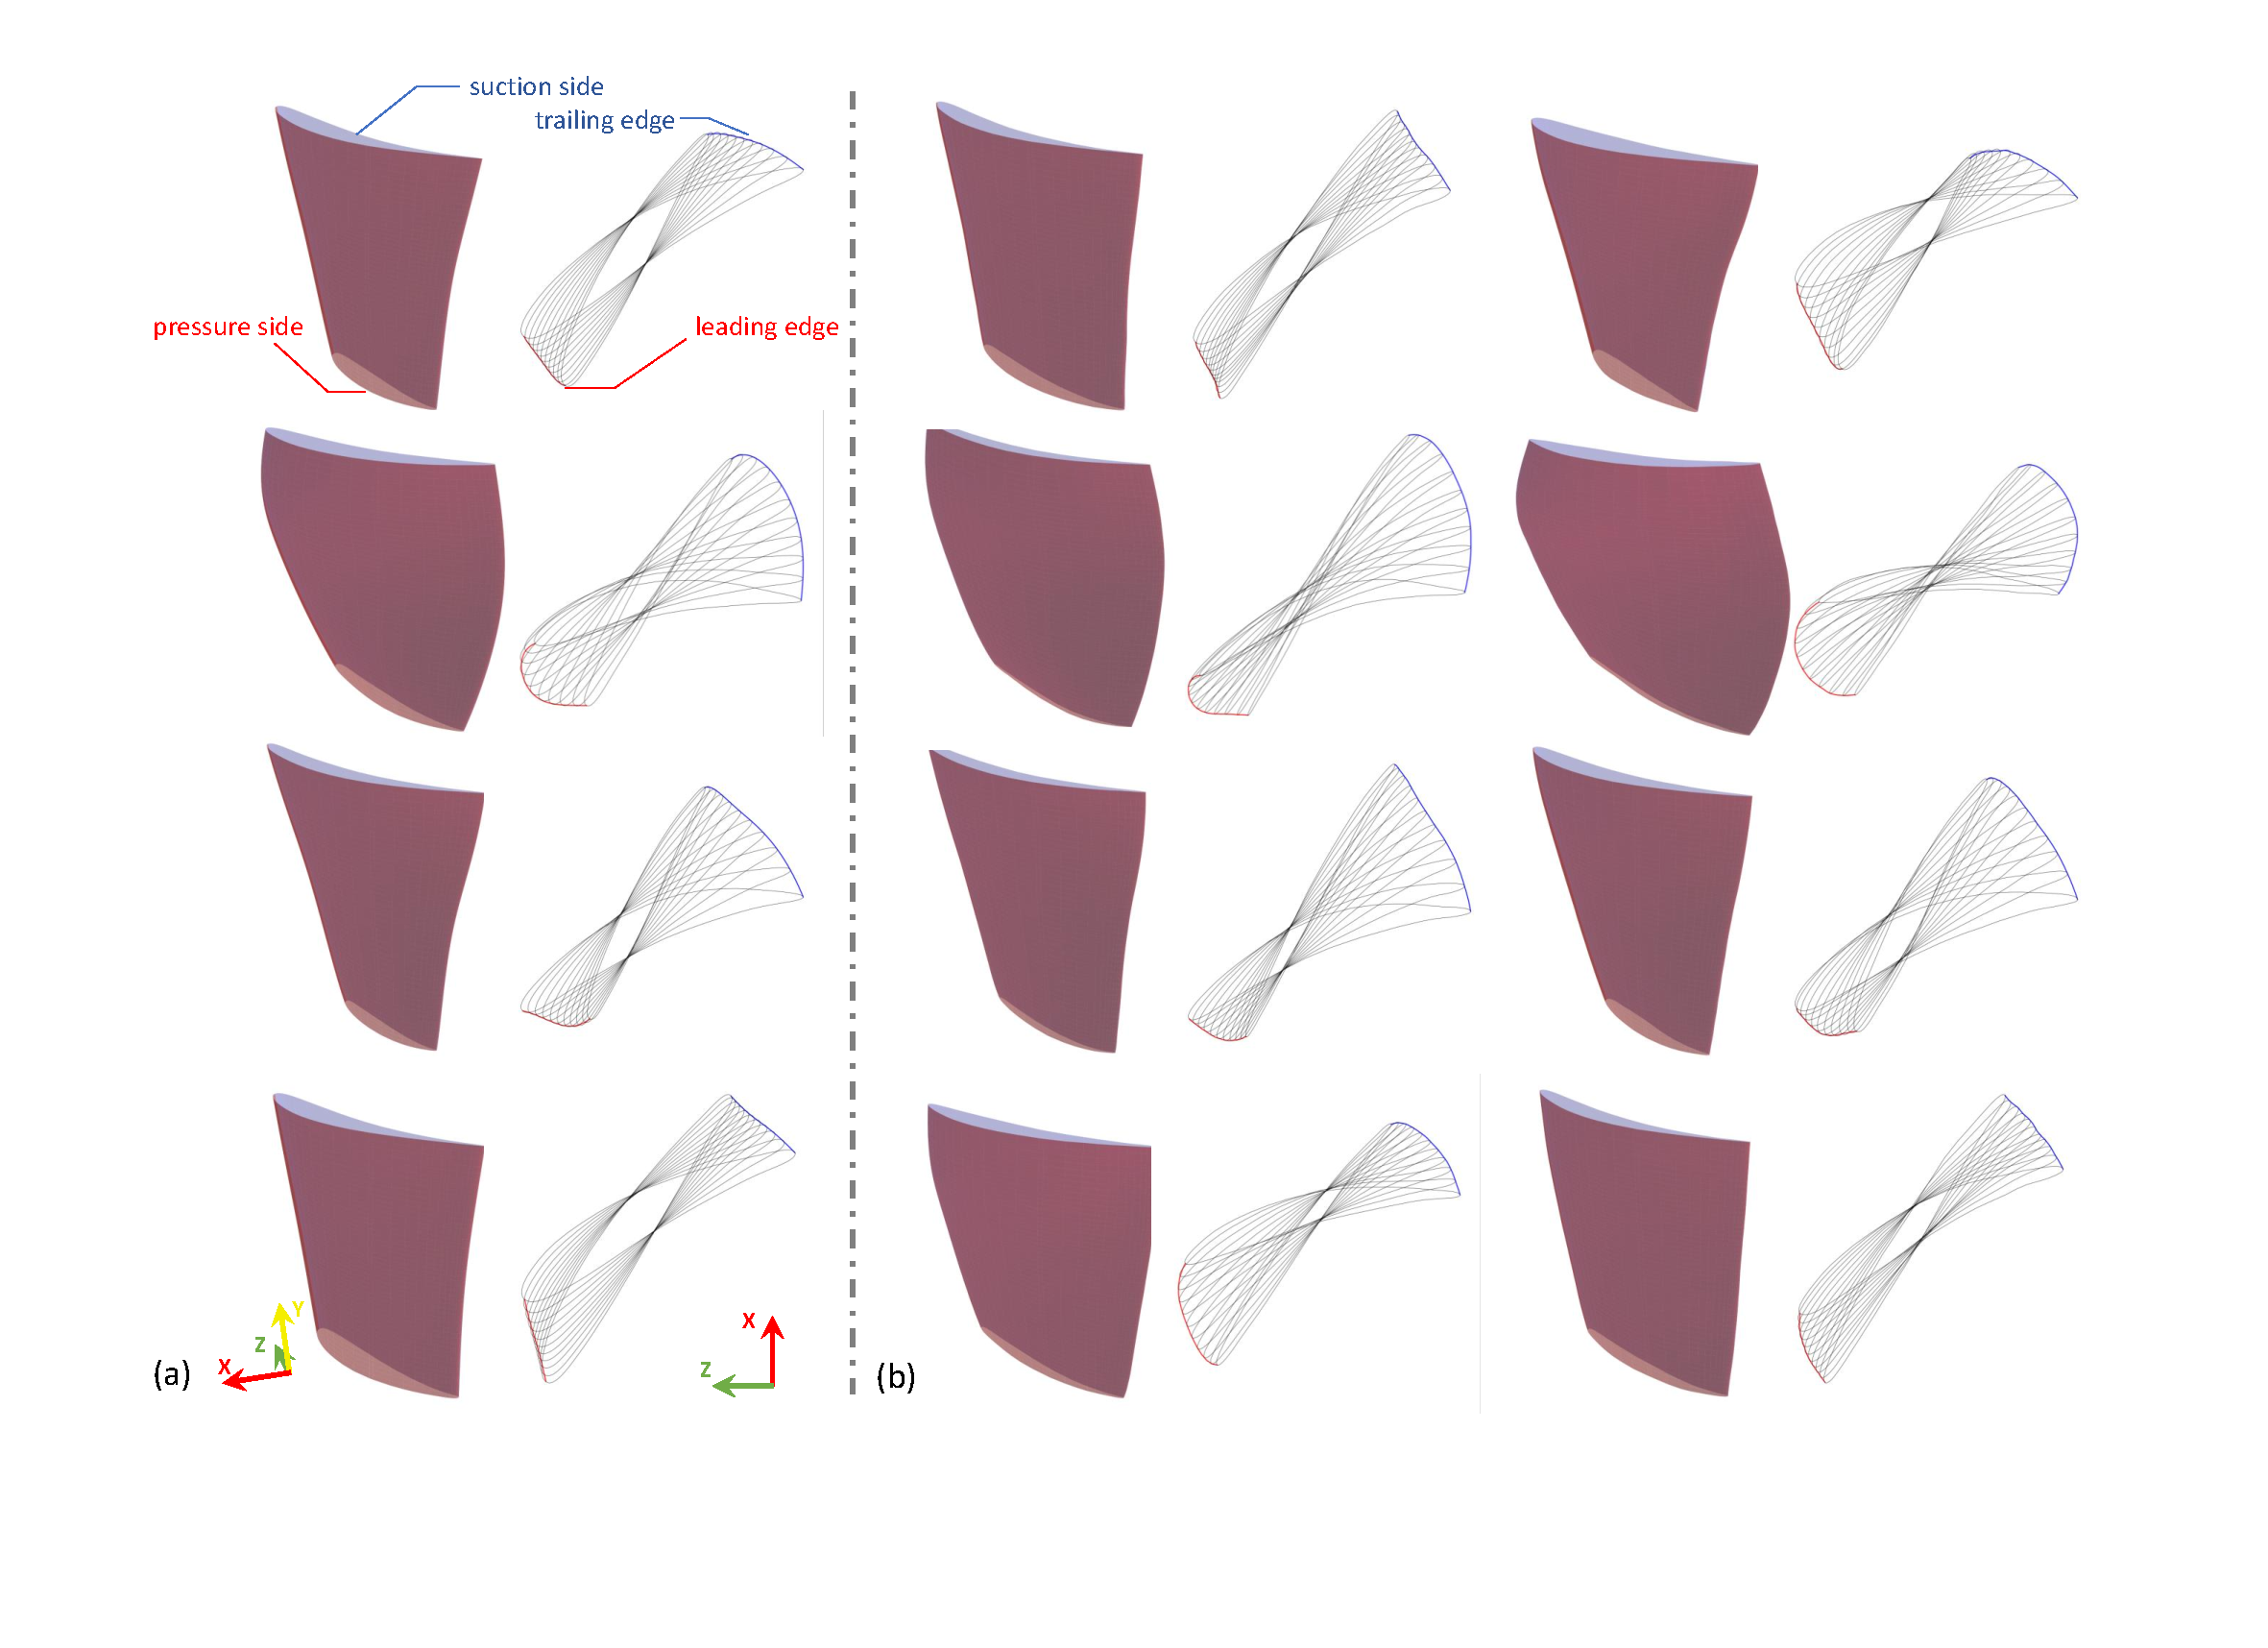
\includegraphics[width=1\linewidth]{chapter6/fig/fig_unconditional_blades.pdf}
    \end{center}
    \caption{
        \small 3D and 2D projected sectional views of (a) training dataset blades, (b) unconditionally generated blades by \textit{DiffGeo}.
    }
    \label{ch6:fig:unconditional_blades}
\end{figure}

To ensure these qualitatively valid outputs also match the statistical distribution of the limited training data, several key geometric parameters between 200 \textit{DiffGeo}-generated blades and the 75 training blades are compared. In Fig.~\ref{ch6:fig:blade_stats}(a) plots several metrics for both sets, including the maximum thickness as a percentage of chord, maximum camber, and angles of attack all at the hub and tip sections. The generated blades (orange distribution) highly align with the training blades (blue distribution) for all these metrics. Similarly, Fig.~\ref{ch6:fig:blade_beta}(a-c) overlays the twist angle distributions (leading edge $\beta_1$ and trailing edge $\beta_2$ twist angles) of the training and generated blades. The individual $\beta$ profiles (in light lines) vary, but the averaged twist law of \textit{DiffGeo}'s generation (in orange solid lines)  matches the $\beta$ of mean training set blade (in blue solid lines). In summary, \textit{DiffGeo} matches the in-convex-hull distribution generated by linear combinations of the six base blades. The next subsections demonstrate capabilities beyond linear interpolation, including fine-grained constrained control and out-of-convex-hull exploration.

\begin{figure}[!htb]
    \begin{center}
        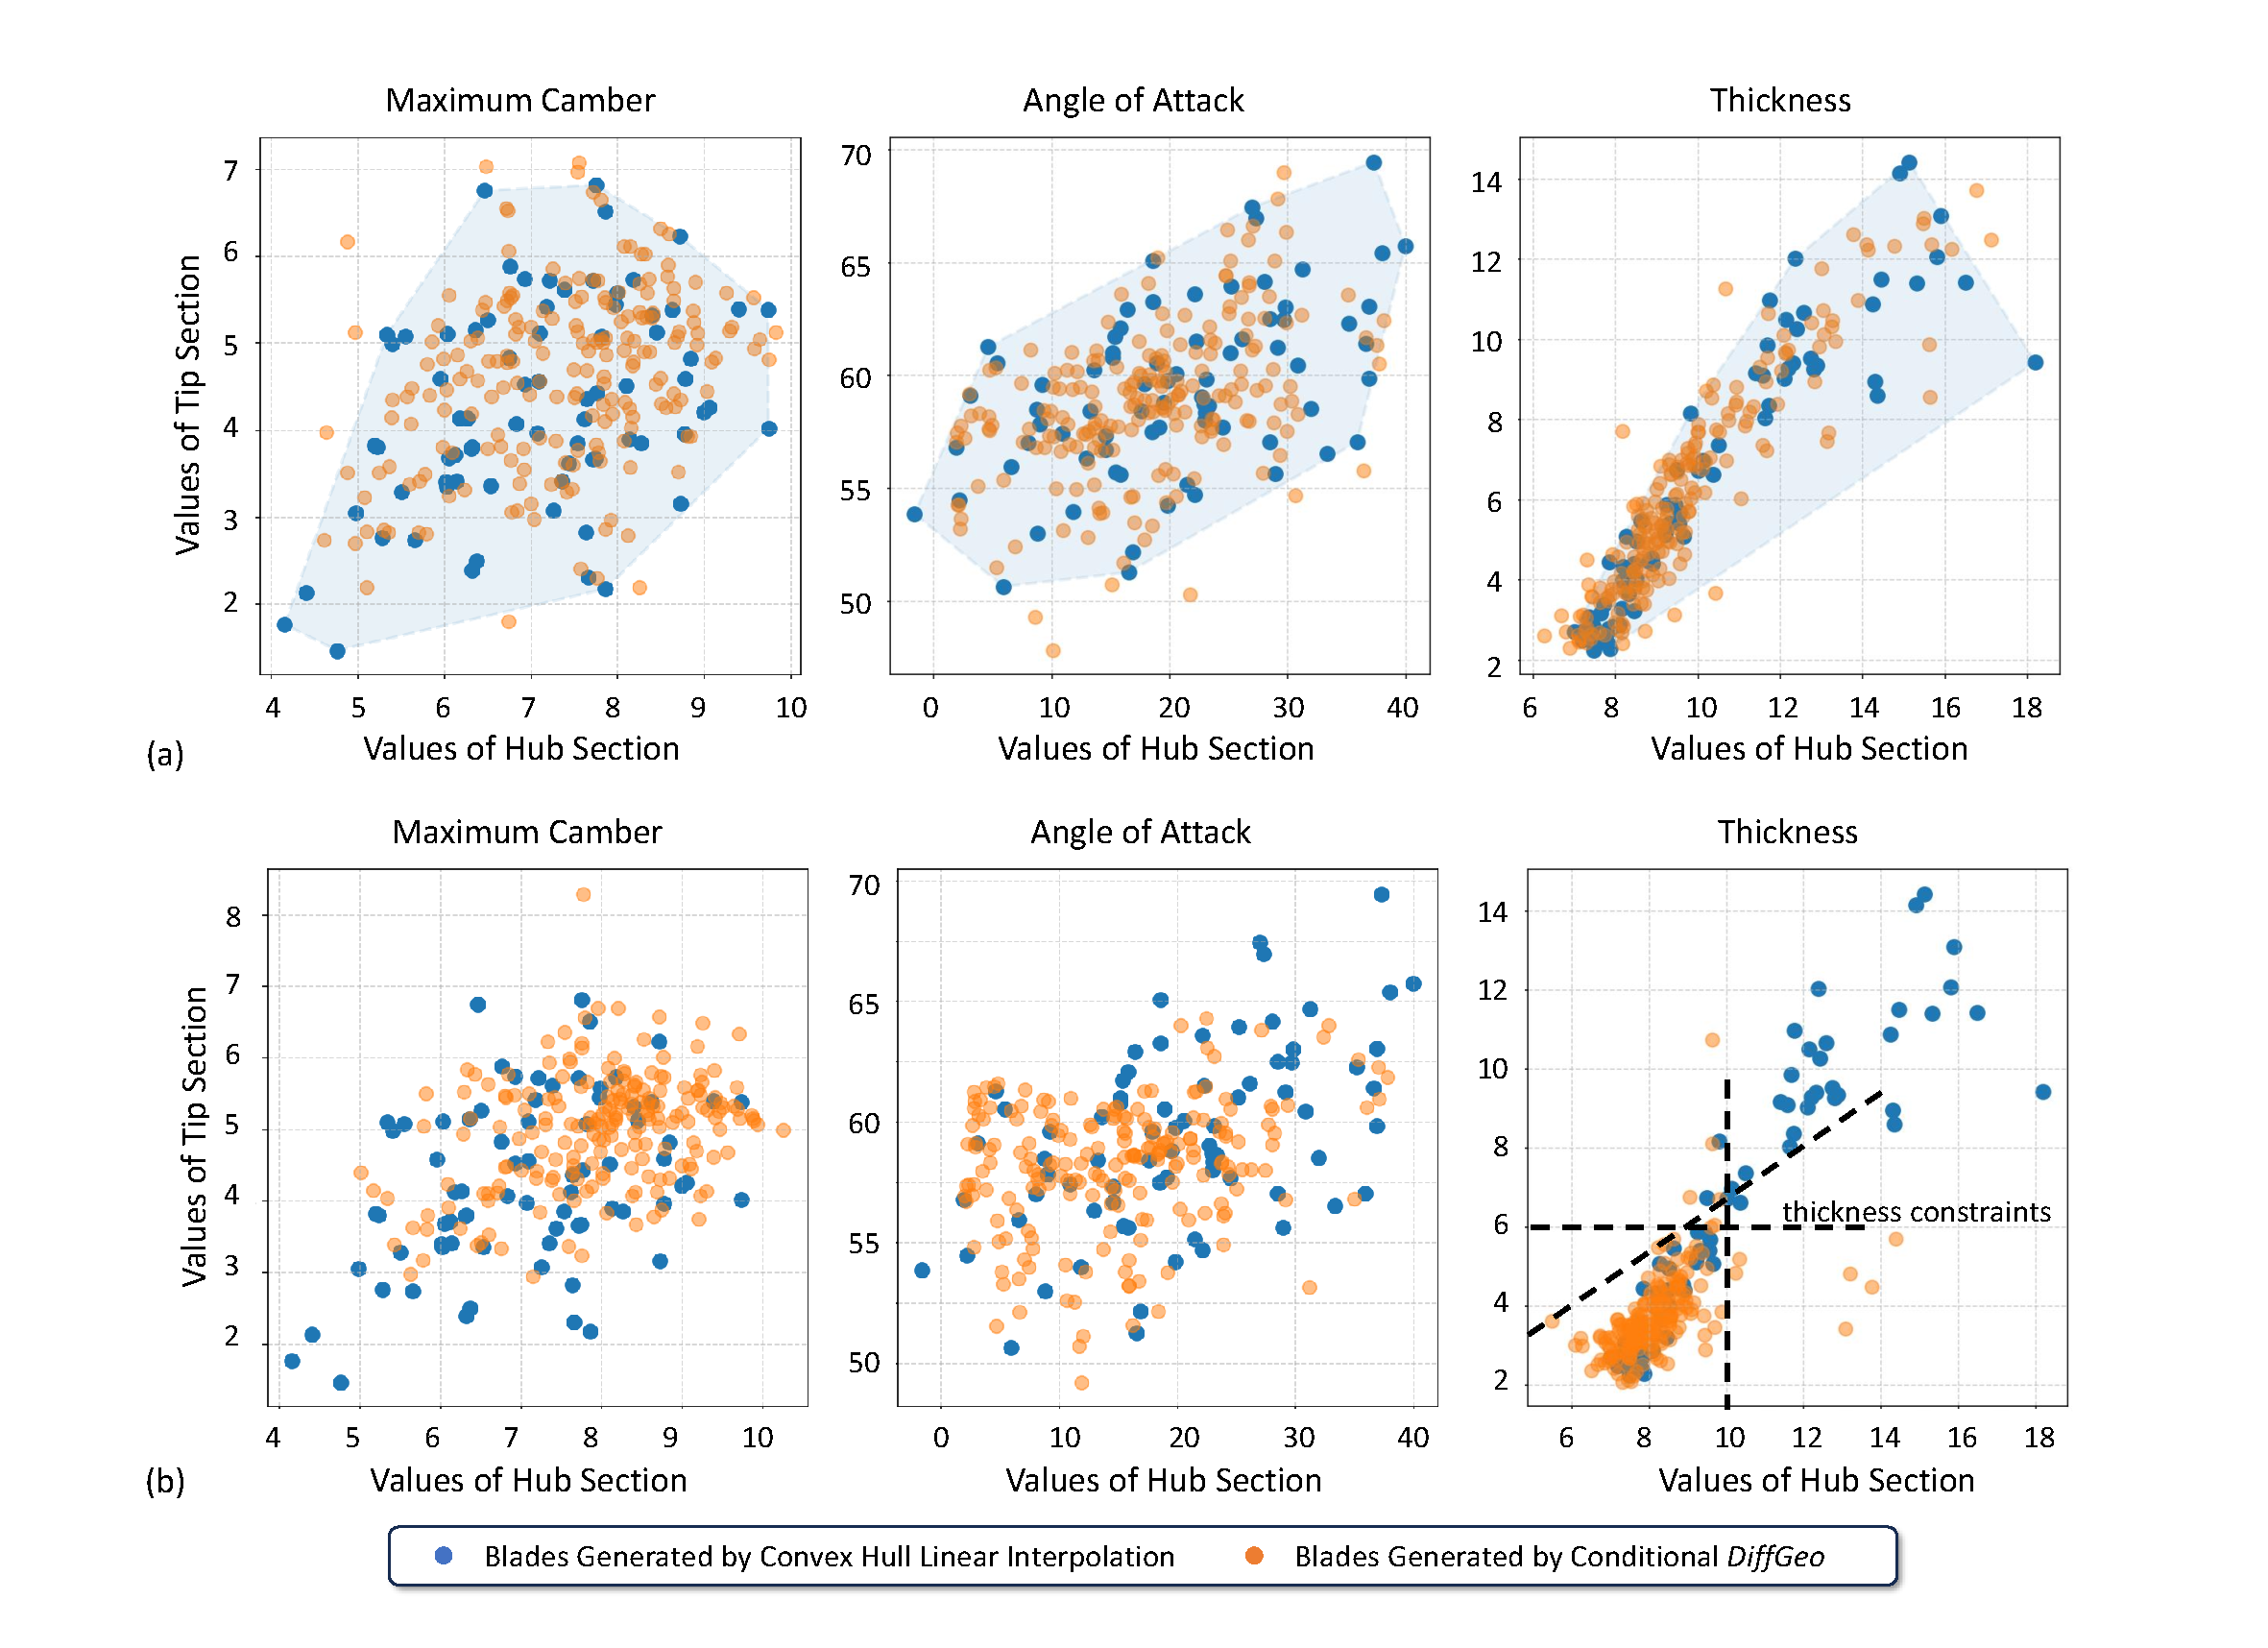
\includegraphics[width=1\linewidth]{chapter6/fig/fig_blade_stats.pdf}
    \end{center}
    \caption{
        \small Geometric statistics of blades by (a) unconditional and (b) conditional \textit{DiffGeo}.
    }
    \label{ch6:fig:blade_stats}
\end{figure}

\begin{figure}[!htb]
    \begin{center}
        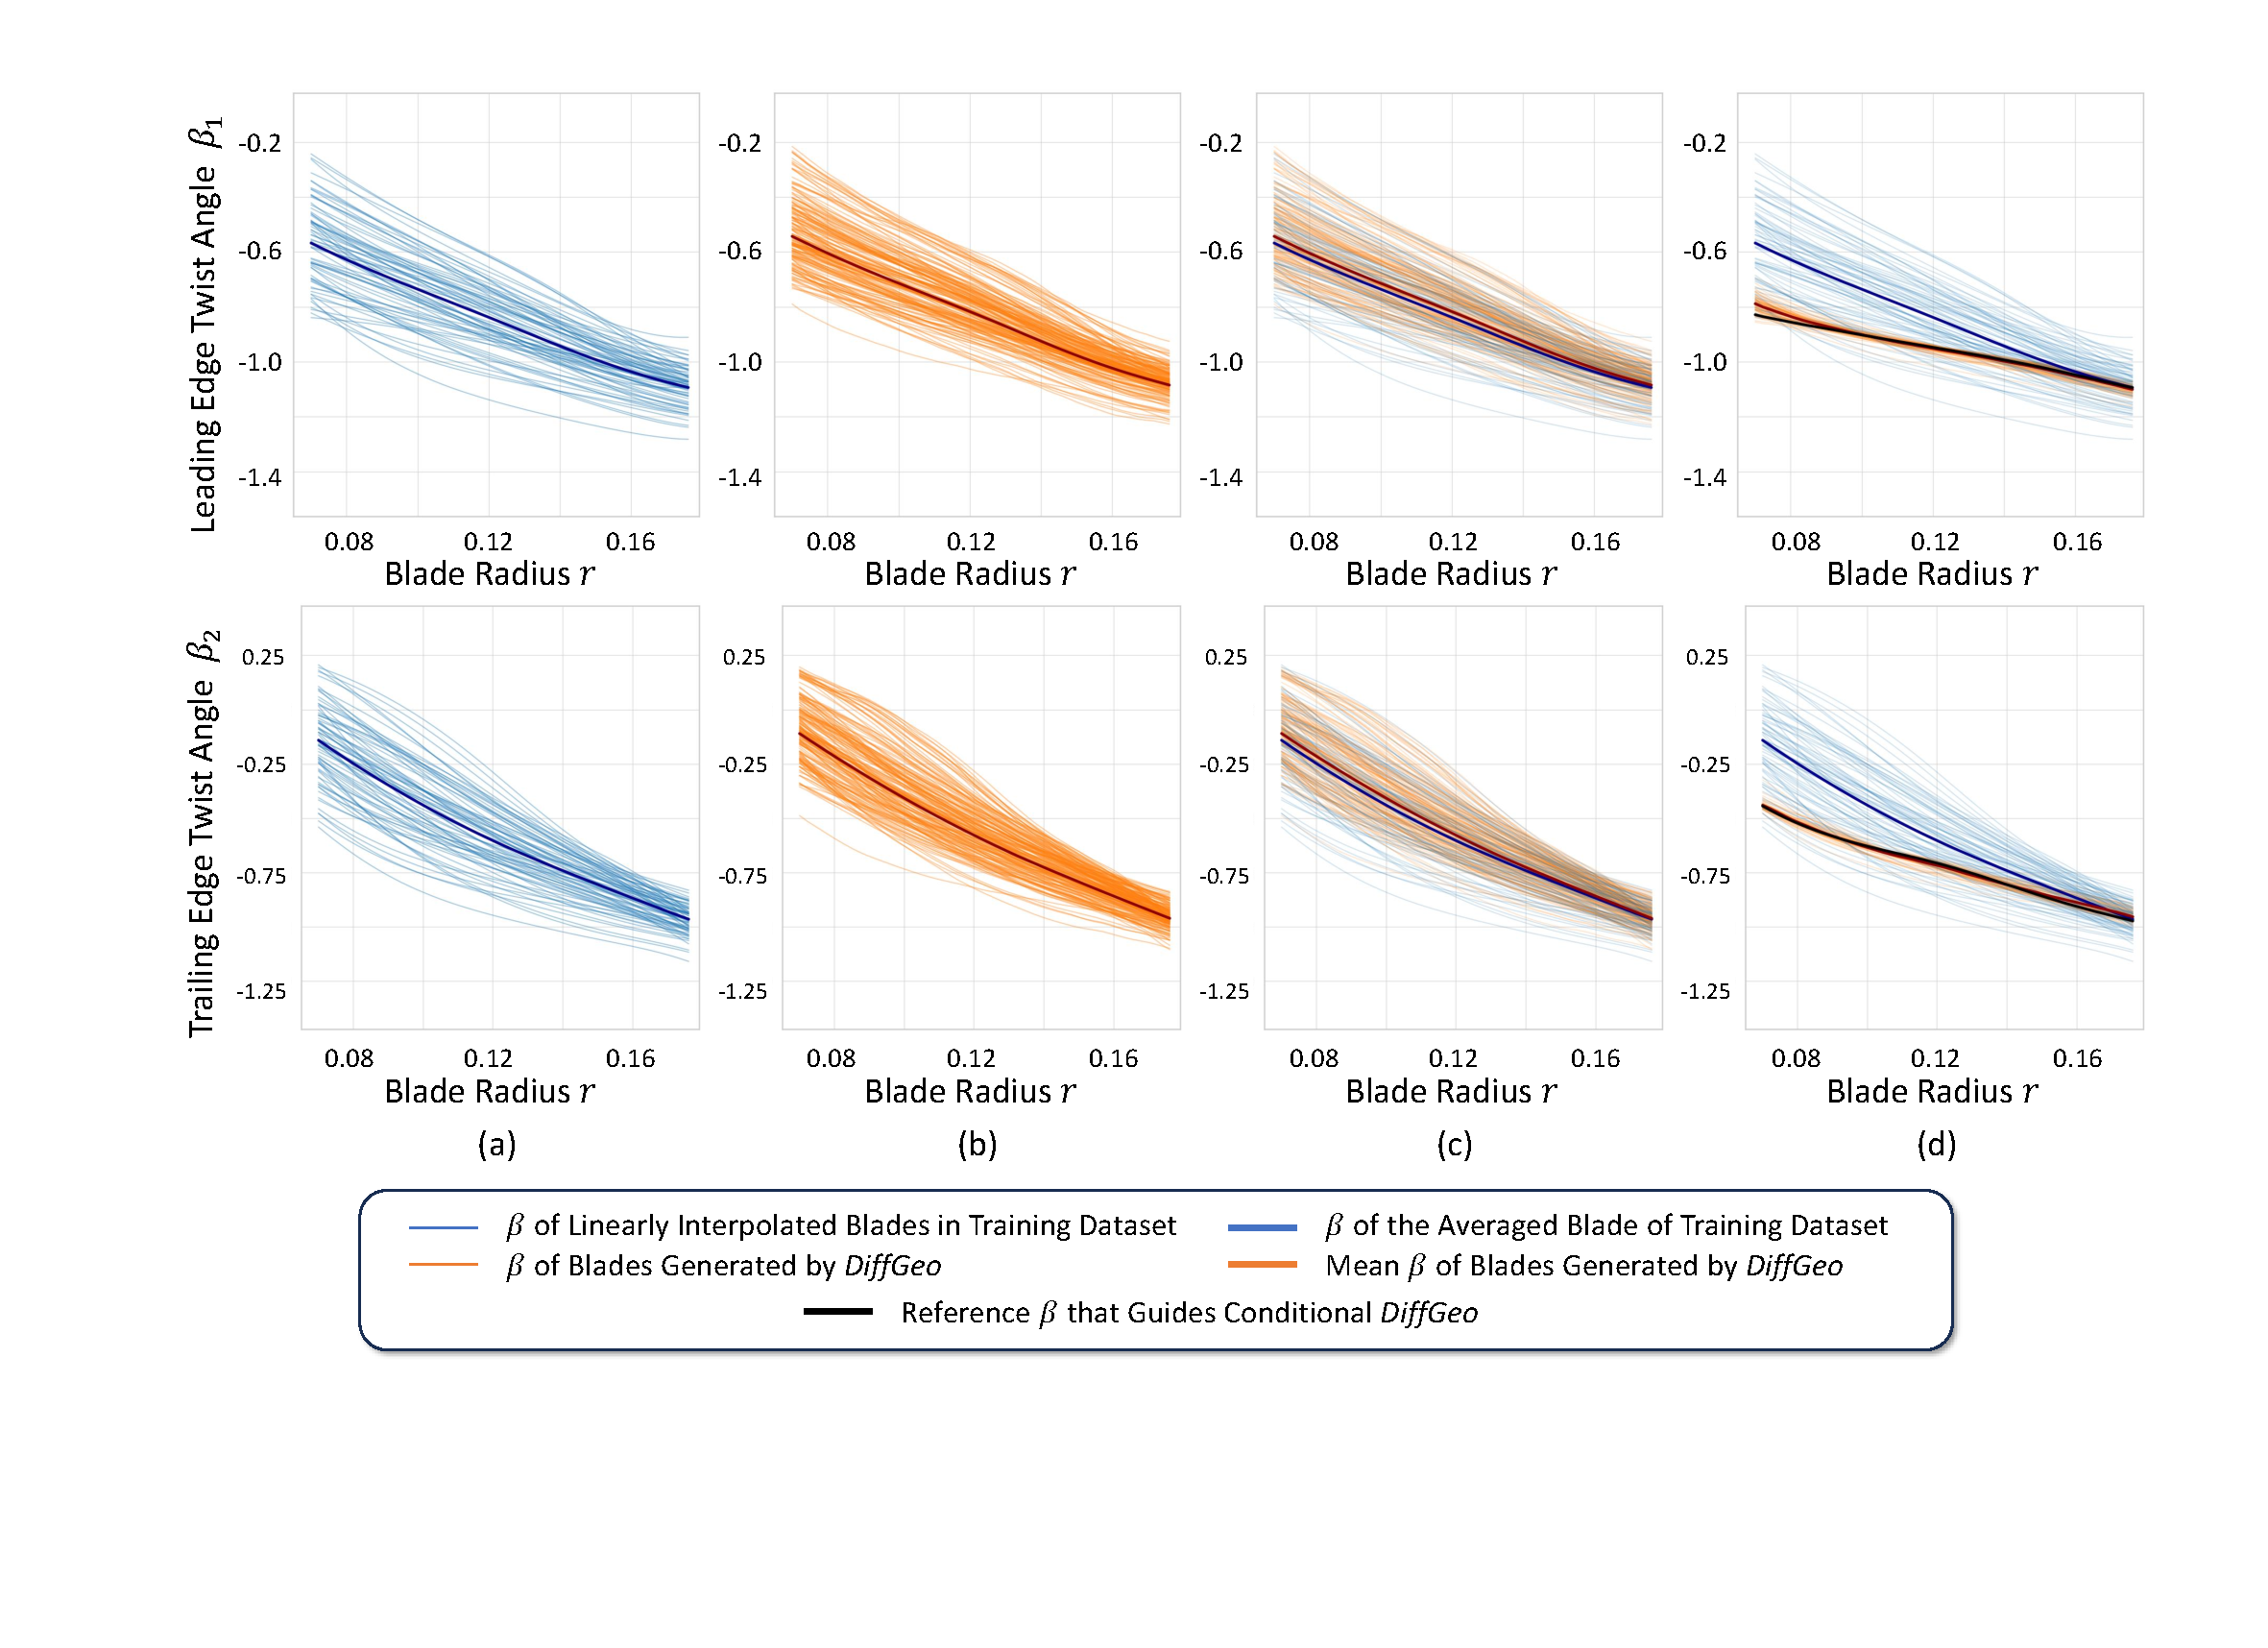
\includegraphics[width=1\linewidth]{chapter6/fig/fig_blade_beta.pdf}
    \end{center}
    \caption{
        \small Blade twist distributions: (a) training dataset, (b) unconditional \textit{DiffGeo}, (c) dataset vs. unconditional \textit{DiffGeo}, (d) dataset vs. twist-guided conditional \textit{DiffGeo}.
    }
    \label{ch6:fig:blade_beta}
\end{figure}

\begin{figure}[!htb]
    \begin{center}
        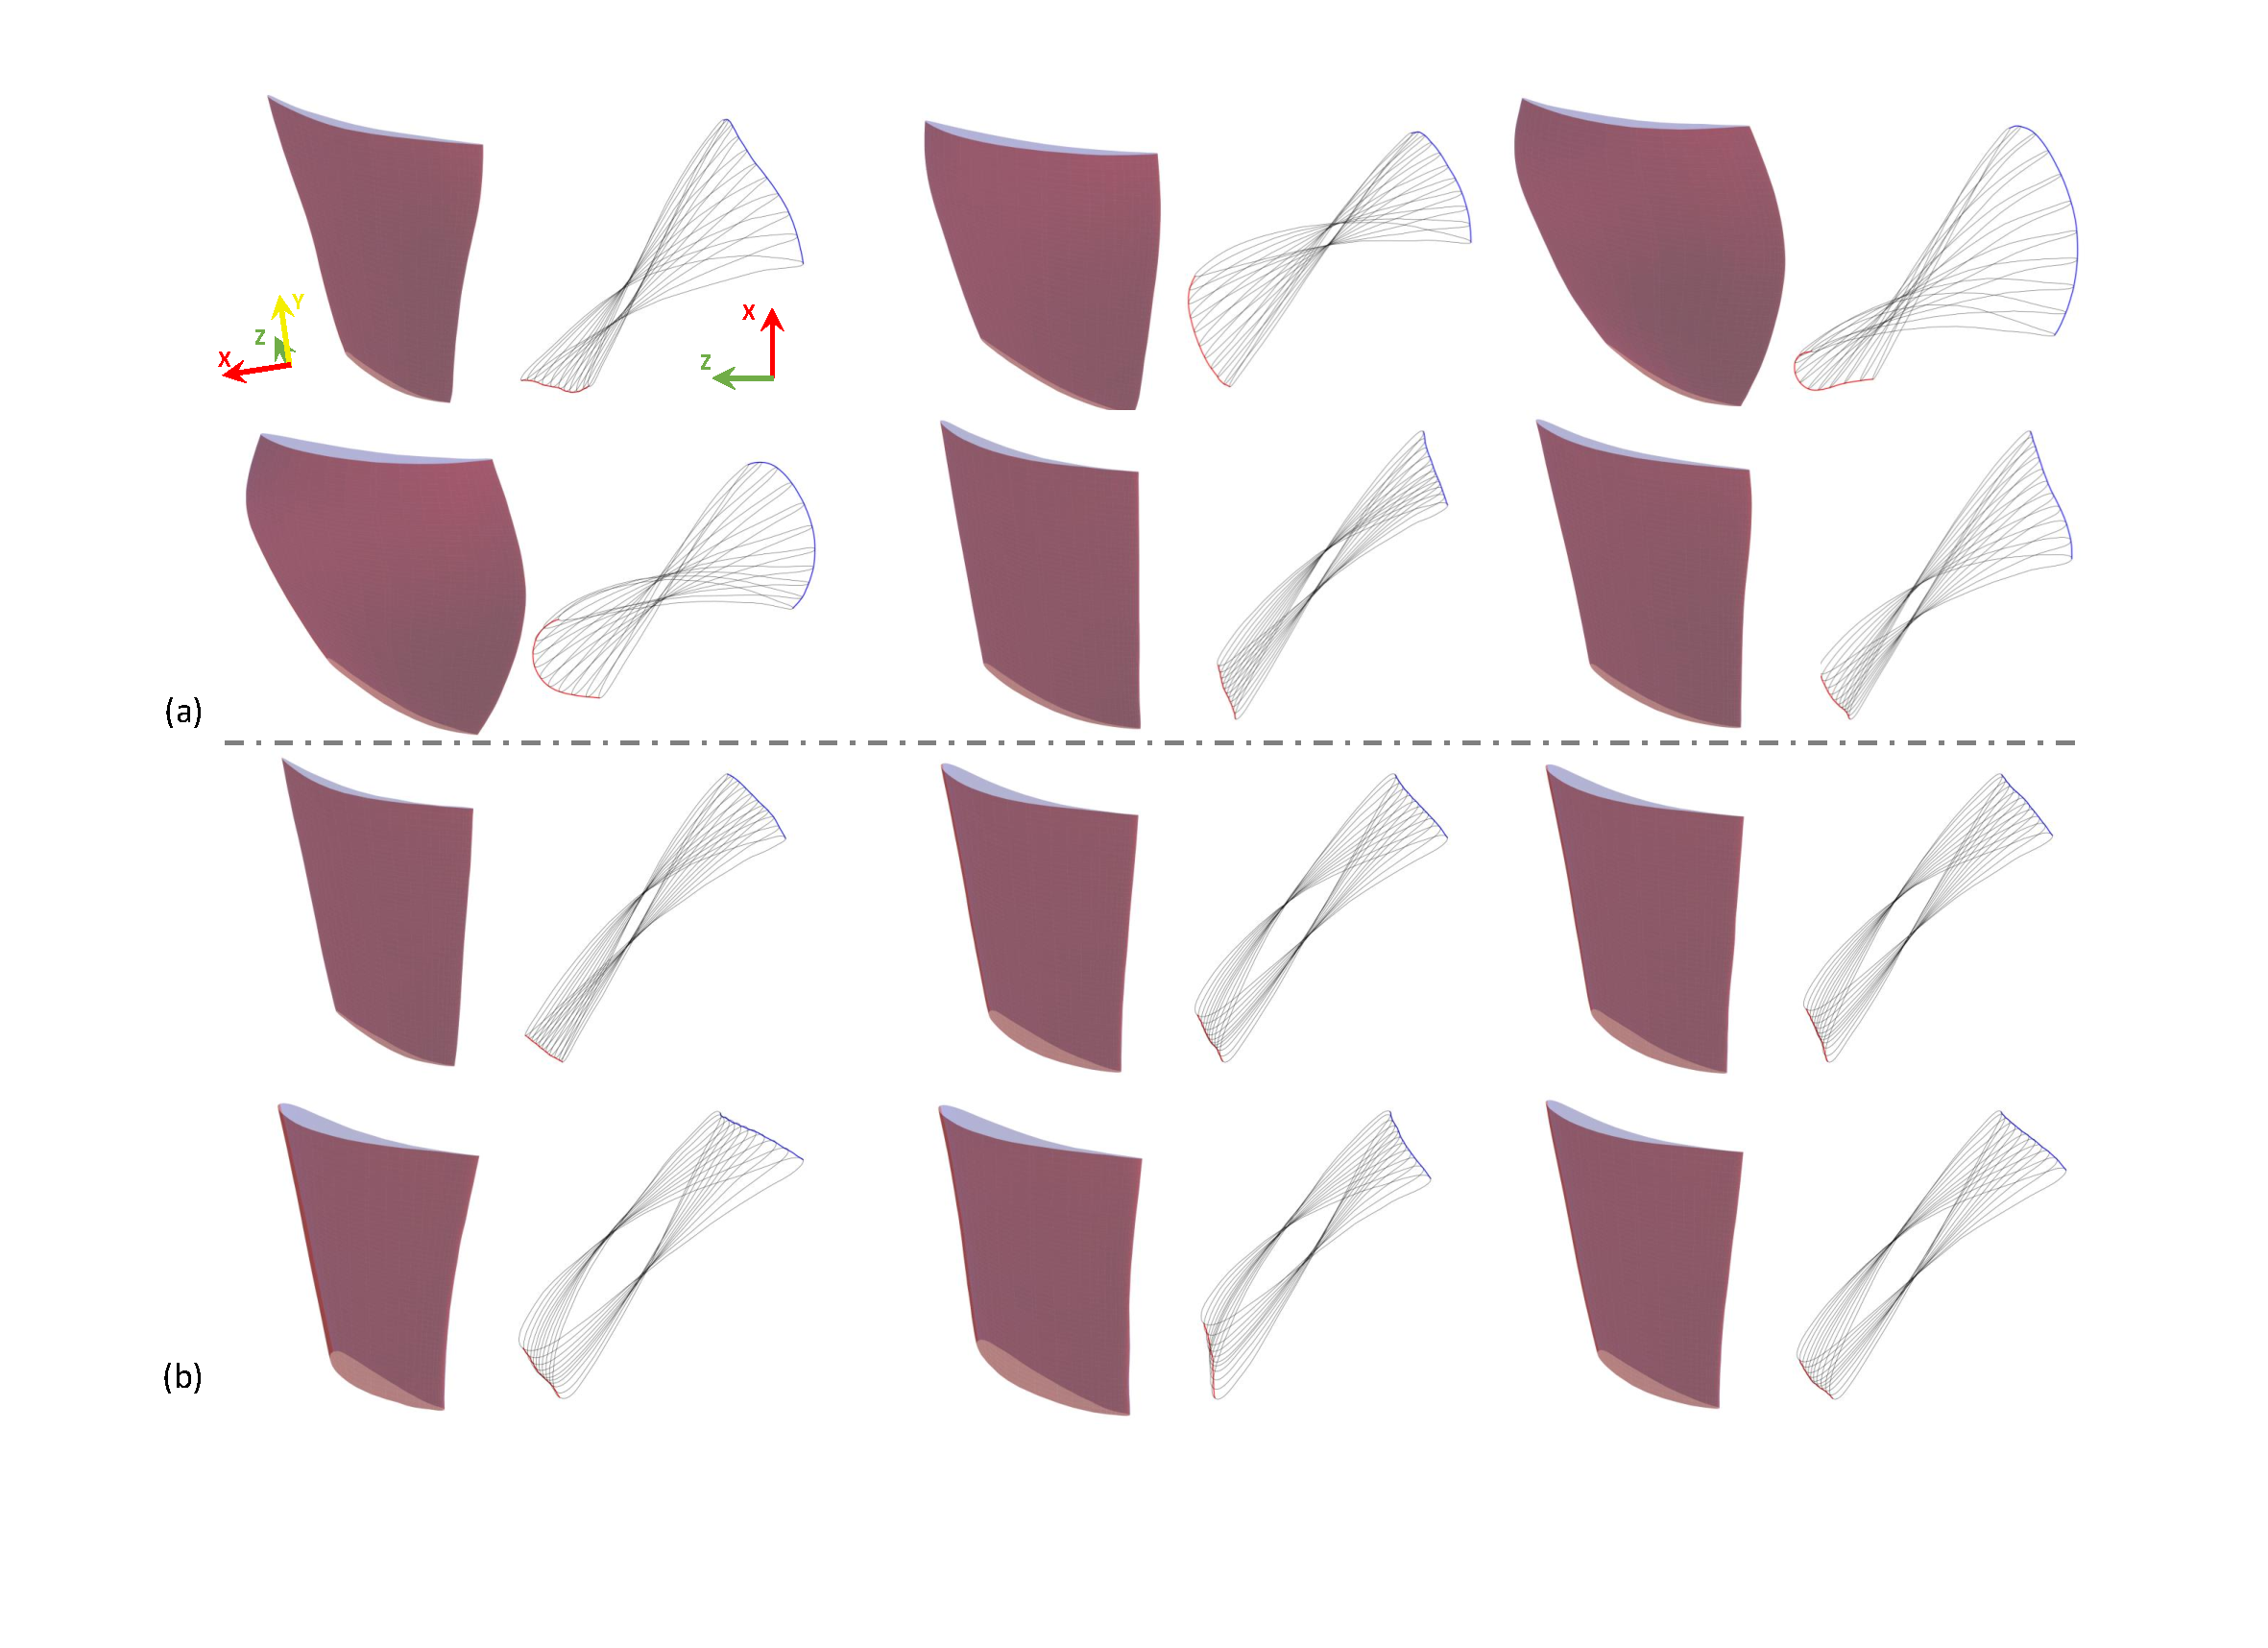
\includegraphics[width=1\linewidth]{chapter6/fig/fig_conditional_blades.pdf}
    \end{center}
    \caption{
        \small 3D and 2D projected sectional views of conditional \textit{DiffGeo} blades guided by (a) thickness constraints, (b) reference twist law.
    }
    \label{ch6:fig:conditional_blades}
\end{figure}

\subsubsection{Controllability of Guided Sampling}
In this section, we investigate \textit{DiffGeo}'s controllability on a 3D task by imposing multiple simultaneous constraints. Specifically, we guide \textit{DiffGeo} to generate blades that satisfy certain thickness requirements at both hub and tip. This simulates an engineering scenario where the blade must meet thickness criteria at different span locations for structural or performance considerations. Three inequality constraints are imposed in the normalized scale of dataset: (i) the hub section’s maximum thickness must be less than 10, (ii) the tip section’s max thickness less than 6, and (iii) the ratio of tip thickness to hub thickness less than $2/3$. These constraints are higher-dimensional and coupled, and are challenging to handle with traditional design of experiments or GAN/VAEs without specialized training. However, they reflect more realistic design rules in turbomachinery.

To integrate these requirements within \textit{DiffGeo}, let $\cT_{hub}(x)$ and $\cT_{tip}(x)$ denote the thickness distributions along the chord for the hub and tip cross-sections of a blade, similar to 2D case. Let:
\begin{align}
    C^I_{hub} &= \max (\max_x \cT_{hub}(x)-10, 0) \;, \\
    C^I_{tip} &= \max (\max_x \cT_{tip}(x)-6, 0) \;, \\
    C^I_{t2h} &= \max (\frac{\underset{x}\max \cT_{hub}(x)}{\underset{x}\max \cT_{tip}(x)}- \frac{2}{3}, 0) \;,
\end{align}
which we sum into a simple composite inequality constraint function $C^I = C^I_{hub} + C^I_{tip} + C^I_{t2h}$. Blades are then generated following the guided sampling steps described in Algorith~\ref{ch6:alg:abs_sample_conditional_diffusion}, where $C^I$ is added as in Equation~\ref{ch6:eq:energy_guidance} to push the generated shape toward satisfying all three thickness limits simultaneously.

Some qualitative results are shown in Fig.~\ref{ch6:fig:conditional_blades}(a). The blade geometries remain smooth and continuous, and patterns such as camber and twist distribution are still diverse, showing valid properties. They exhibit visibly thinner profiles at the tip and/or hub compared to unconditional generated samples. Fig.~\ref{ch6:fig:blade_stats}(b) quantitatively demonstrates the effect of thickness constraints for 200 guided samples (in orange points), where the thickness metrics have clearly shifted while the other metrics, including camber and angle of attacks ($AoA$), remain aligned with the training data (in blue points). \textit{DiffGeo} successfully isolates the effect of enforcing thickness constraints as it generates new shapes that fulfill the constraints without distorting unrelated aspects of the blade geometry. This highlights \textit{DiffGeo}’s ability to handle high-dimensional constraints, achieving results results that would be intractable for brute-force sampler or retrained models under limited data.

\subsubsection{Nonlinear Exploration Beyond Linear Interpolation}
A central question for this case study is whether \textit{DiffGeo} can produce truly novel blades that are not simply interpolations of the limited training set. Since the training blades lie in the convex hull of six existing designs, any design outside that convex hull represents a nonlinear combination or extrapolation that introduces new geometry. 

To answer this question quantitatively, we perform a linear reconstruction error analysis. Let the six base blades be $\{S_1,...,S_6\}$, the interpolated training data be $\{\bar{S}_1,...,\bar{S}_{75}\}$ and $K$ generated blades be $\{M_1,...,M_K\}$. The reconstruction errors of training dataset $\mathcal{E}_{data}$ and of \textit{DiffGeo}'s generation $\mathcal{E}_{gen}$ are defined as the solutions to the following optimization problems:
\begin{align}
    \mathcal{E}_{data}^{(i)} & =\underset{\{w_1^{(i)},...,w_6^{(i)}\}} {\mathrm{min}} \frac{1}{75}\sum_{j=1}^{75} \bigl\| \bar{S}_j-\sum_{k=1}^6 w_k^{(i)}S_k \bigr\|^2 \;,\\
    \mathcal{E}_{gen}^{(i)} & =\underset{\{w_1^{(i)},...,w_6^{(i)}\}} {\mathrm{min}} \frac{1}{K}\sum_{j=1}^{K} \bigl\| M_j-\sum_{k=1}^6 w_k^{(i)}S_k \bigr\|^2 \;,
\end{align}
where $\{w_1^{(i)}, \dots, w_6^{(i)}\}$ are nonnegative interpolation weights for the $i$-th tested blade subject to $\sum_{j=1}^6 w_j = 1$, ensuring each reconstruction lies within the convex hull of the base blades. A higher reconstruction error indicates a greater deviation from the linear subspace and reflects stronger nonlinearity in the blade geometry.

By definition, the training blades have near-zero reconstruction error, which is confirmed in Fig.~\ref{ch6:fig:linearity_check}.
In comparison, \textit{DiffGeo}-generated blades show substantially larger convex-hull residuals: 9.7 for unconditional generation and 24.9 for thickness-guided generation, measured as the average per-surface-point L2 distance. For reference, the typical hub-section chord length is about 80, meaning these residuals correspond to roughly $12\%$ and $31\%$ of the hub chord, respectively. Such magnitudes are well beyond numerical tolerance, indicating that the generated blades cannot be represented by any convex combination of the six bases, and that \textit{DiffGeo} explores geometry outside the range accessible to linear interpolation.

\begin{figure}[!htb]
    \begin{center}
        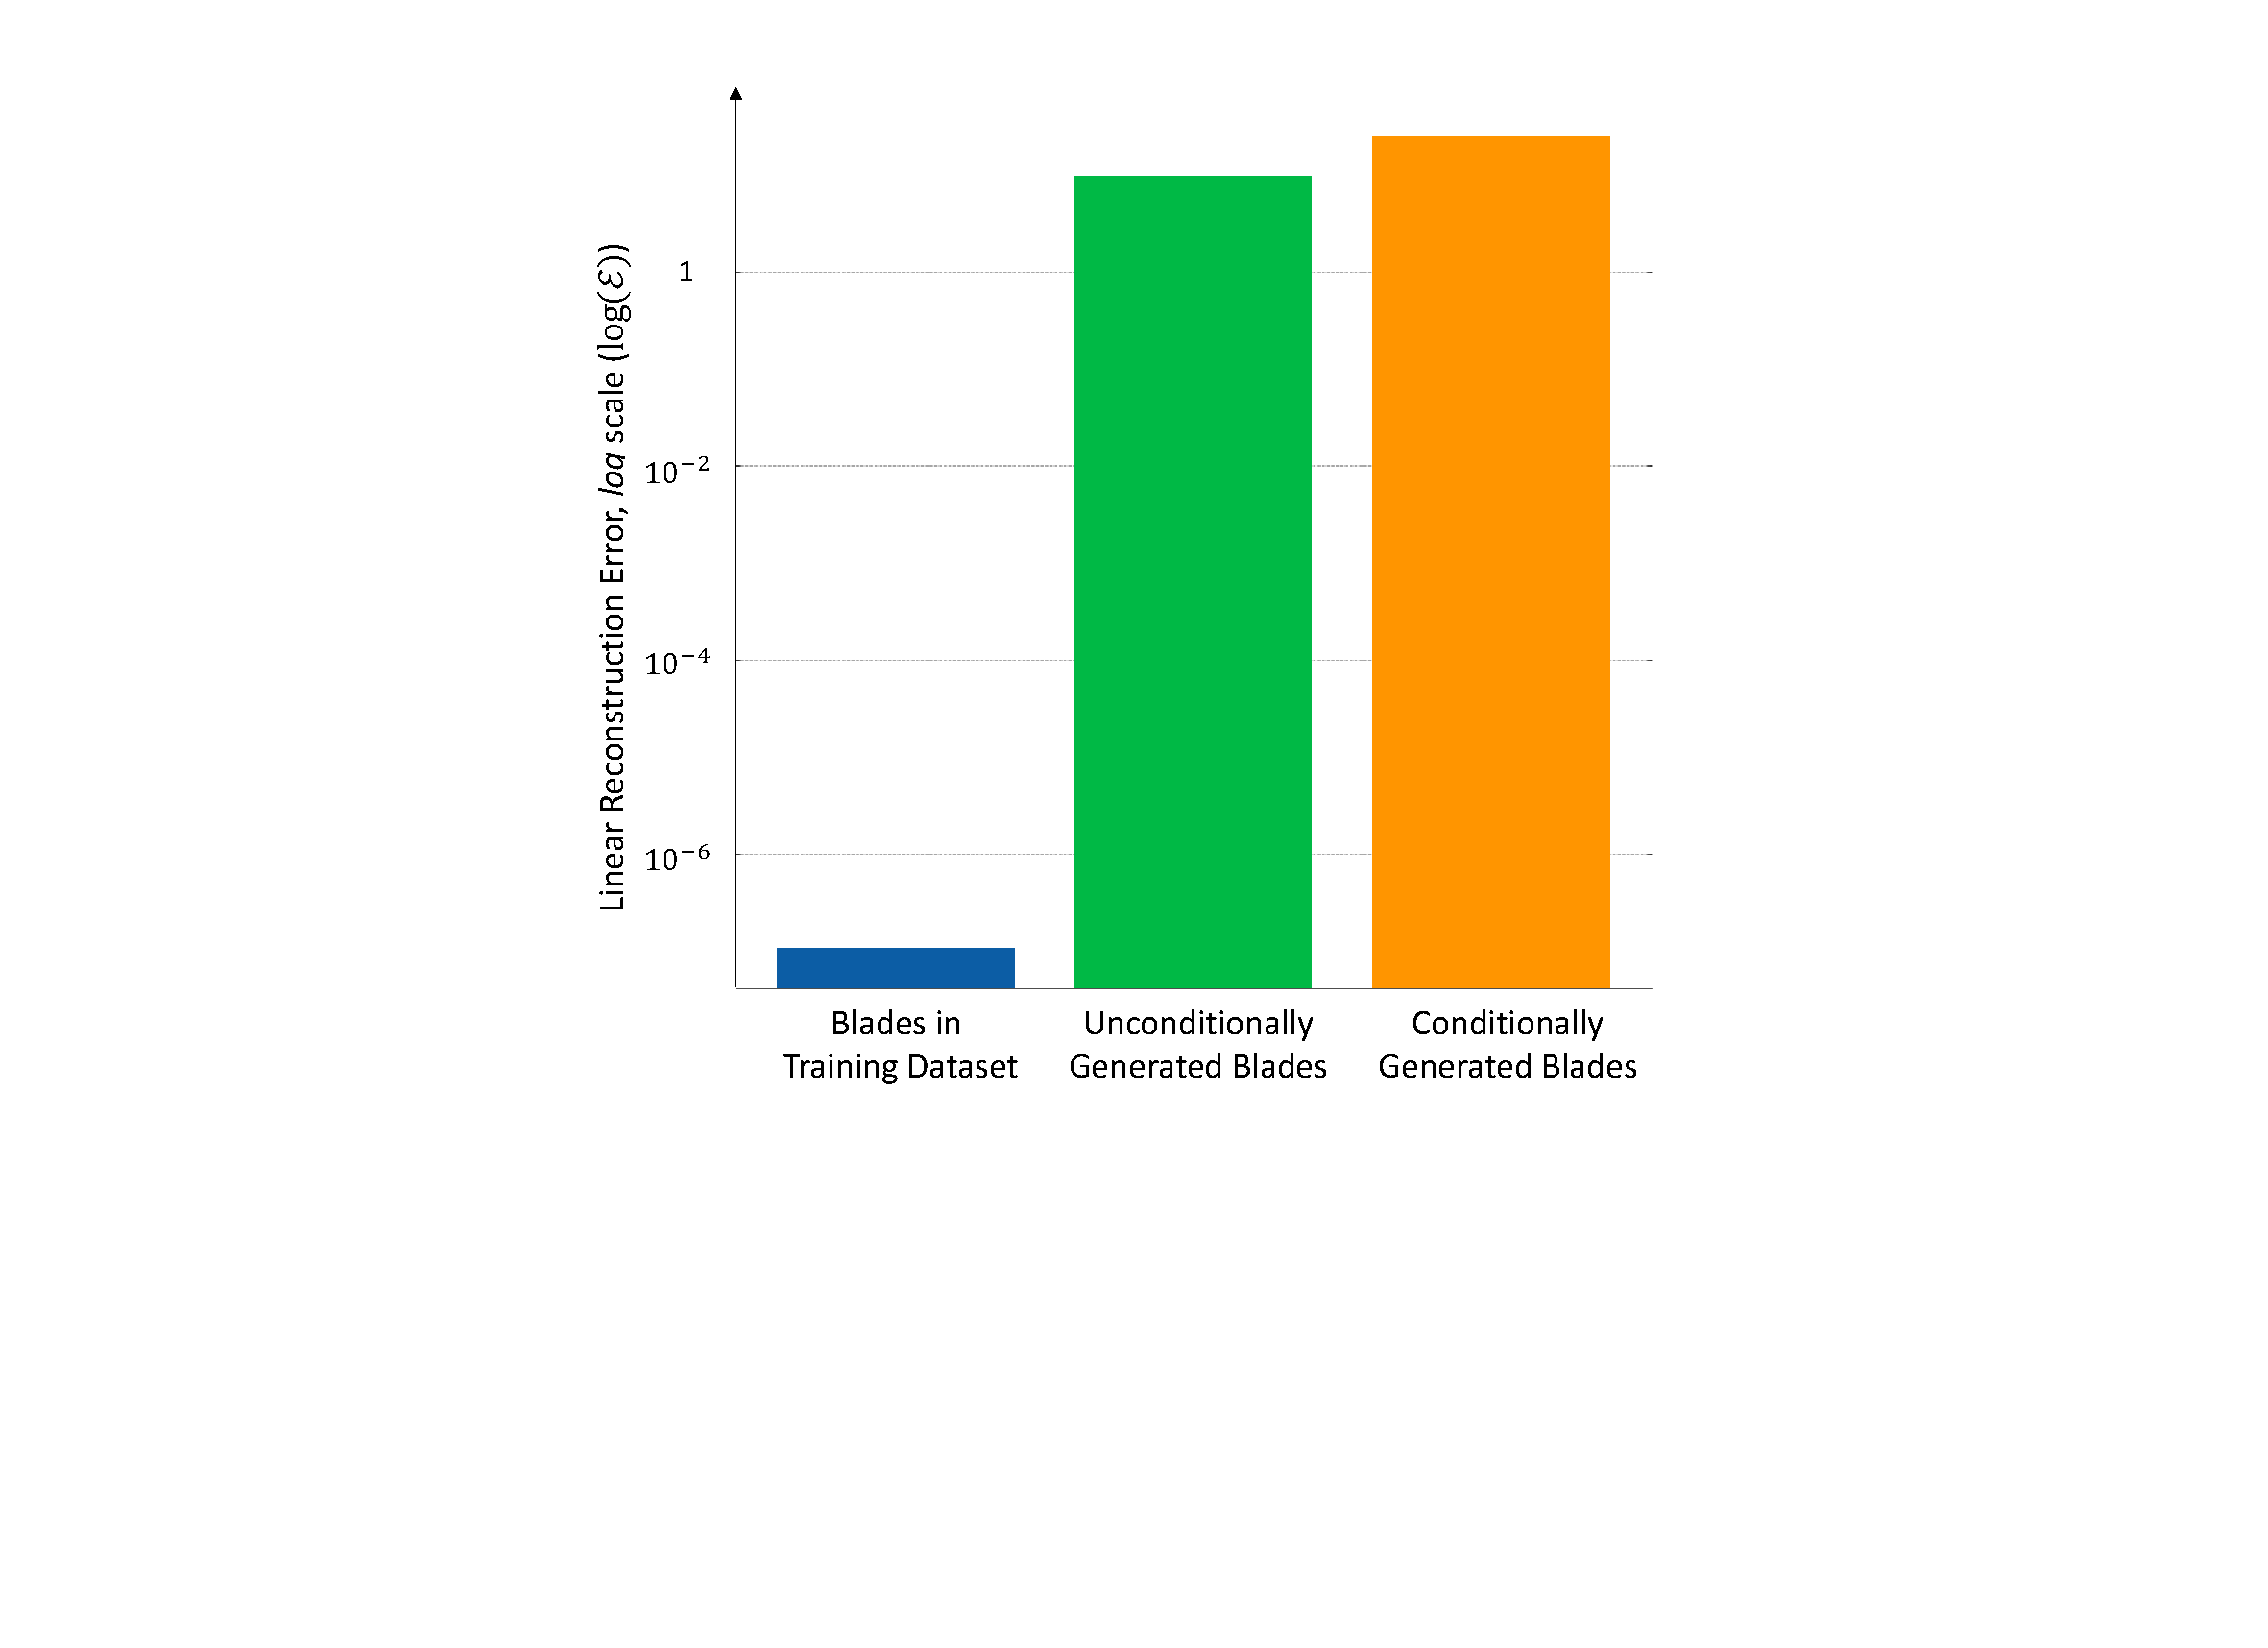
\includegraphics[width=1\linewidth]{chapter6/fig/fig_linearity_check.pdf}
    \end{center}
    \caption{
        \small Linear reconstruction errors of (a) interpolated dataset blades, (b) \textit{DiffGeo} unconditional outputs, (c) thickness-guided conditional outputs.
    }
    \label{ch6:fig:linearity_check}
\end{figure}

To further evaluate nonlinear conditional controllability, we compare \textit{DiffGeo} with the linear convex interpolation under a new set of design constraints. Specifically, we define four  specifications: hub maximum thickness of 12, tip maximum thickness of 8, hub angle of attacks of $10^{\circ}$ and tip angle of attacks of $55^{\circ}$. As can be observed in Fig.~\ref{ch6:fig:blade_stats}, each specification lies well within the convex hull spanned by the six base blades. For \textit{DiffGeo}, we apply energy-based guidance and generate 20 guided samples. For convex interpolation, we optimize nonnegative weights with different random initialization over the six bases to minimize the same energy.

Despite each of the target being in-convex-hull, the linear interpolation struggles to satisfy all constraints simultaneously. The hub AoA incurs a large residual, indicating a strong trade-off between these targets. In contrast, \textit{DiffGeo} achieves balanced and low total error across all specifications. Tab.~\ref{ch6:tab:blade_diffgeo_linear_comparison} shows the quantitative results. In terms of generation diversity, linear interpolation's mean standard deviation across surface points is $0.31$, while \textit{DiffGeo} produces a larger mean standard deviation of $1.40$ under the same target. This comparison clearly demonstrates that \textit{DiffGeo}’s nonlinear latent space offers additional degrees of freedom for DSE than linear convex interpolation, while maintaining geometric validity and without sacrificing sample diversity.

\begin{table}[htbp]
  \centering
  \caption{Constraint errors of conditional generations under in-convex-hull target using \textit{DiffGeo} and linear convex interpolation.}
  \resizebox{\textwidth}{!}{
    \begin{tabular}{lccccc}
    \hline
    DSE Methods & \multicolumn{1}{l}{Error of $\cT_{hub}$} & \multicolumn{1}{l}{Error of $\cT_{tip}$} & \multicolumn{1}{l}{Error of ${AoA}_{hub}$} & \multicolumn{1}{l}{Error of ${AoA}_{tip}$} & \multicolumn{1}{l}{Total Error}\\
    \hline
    \textit{DiffGeo} & 1.037  & 0.573  & 0.448  & 0.629  & 2.687\\
    Linear Convex Hull & 0.018  & 0.578  & 6.353  & 0.859  & 7.808\\
    \hline
    \end{tabular}%
  }
  \label{ch6:tab:blade_diffgeo_linear_comparison}%
\end{table}%

\subsubsection{Integrating \textit{DiffGeo} with Mean-Line Design}
Finally, we show how \textit{DiffGeo} can interface with a conventional mean-line design tool to streamline 3D blade prototyping. The mean-line design offers a fast and analytical means of exploring preliminary performance. A typical design workflow for a new rotor blade starts with global specifications, including expected mass flow rate, pressure ratio and rotational speed. Then the mean-line design tool performs one-dimensional through-flow analysis to solve conservation equations along a representative stream surface between hub and shroud, which produces spanwise distributions of key aerodynamic quantities, including flow angles, blade loading and annulus areas. A key output is the spanwise twist law $\beta$, which prescribes the blade metal angle from hub to tip, and ensures proper incidence and work distribution across the rotor. Along with the chord and solidity distributions, $\beta$ defines a family of quasi-3D sections from which the blade geometry can be reconstructed. Designers then create a 3D blade geometry that realizes this twist and meets other loading criteria, often by manually adjusting and stacking 2D airfoil sections which is a time-consuming process and a bottleneck for rapid conceptual design exploration. We propose using \textit{DiffGeo} to automate the generation of candidate 3D blade geometries that satisfy the mean-line prescribed twist, thus providing a transformed workflow: instead of manually constructing 3D blades, \textit{DiffGeo} proposes viable candidates to choose from as ready starting points for subsequent CFD-based analysis and optimization. This transition can reduce design complexity and workloads.

In this investigation, we seek to design a single-stage axial rotor at 0.3 mach and sea-level conditions. The design specifications include pressure ratio around 1.59 and rotation speed at 1800 rad/s. The reference twist laws $\hat{\beta}_1$ and $\hat{\beta}_2$ are obtained from an interactive mean-line design software that parameterizes the twist distribution with Bezier curves. The reference $\hat{\beta}_1$ and $\hat{\beta}_2$ are incorporated as guidance in \textit{DiffGeo}'s generation by formulating an energy term $C^E=C_{\beta_1}^E+C_{\beta_2}^2$, where:
\begin{align}
    C_{\beta_1}^E &= \int_{r_h}^{r_t} \bigl\|\hat{\beta}_1(r) - \beta_1(r,M)\bigr\|^2 dr \;, \nonumber \\
    C_{\beta_2}^E &= \int_{r_h}^{r_t} \bigl\|\hat{\beta}_2(r) - \beta_2(r,M)\bigr\|^2 dr \;,
    \label{ch6:eq:beta_constraint}
\end{align}
with $r_h$ and $r_t$ being the hub and tip radii, and $\beta_1(r,M)$ and $\beta_2(r,M)$ the corresponding twist distributions of a generated blade $M$. In practice, we discretize these integrals into sums over 50 spanwise sections. Minimizing $C_E$ during generation will encourage the blade’s twist to follow the mean-line solution.

Because matching an entire twist distribution is a stringent constraint, we apply enhanced conditional sampling as described in Algorithm~\ref{ch6:alg:abs_sample_enhanced_conditional_diffusion} with $N^T=3$ and $T^*=650$ to improve convergence. 300 blades targeted at the reference twist laws are generated, and Fig.~\ref{ch6:fig:conditional_blades}(b) shows some of them. Through the projected view of stacked spanwise sections, these blades have the preferred characteristic twist and still exhibit variability in other aspects like camber and thickness distribution. The $\beta$ distributions of conditional blades are compared in Fig.~\ref{ch6:fig:blade_beta}(d) (in orange lines) with the dataset distribution (in blue lines) and the reference target (in black solid lines). The guided blades indeed closely follow the reference twist law on average, showing that the energy guidance has successfully induced \textit{DiffGeo} to meet the mean-line design output.

\begin{figure}[!tb]
    \begin{center}
        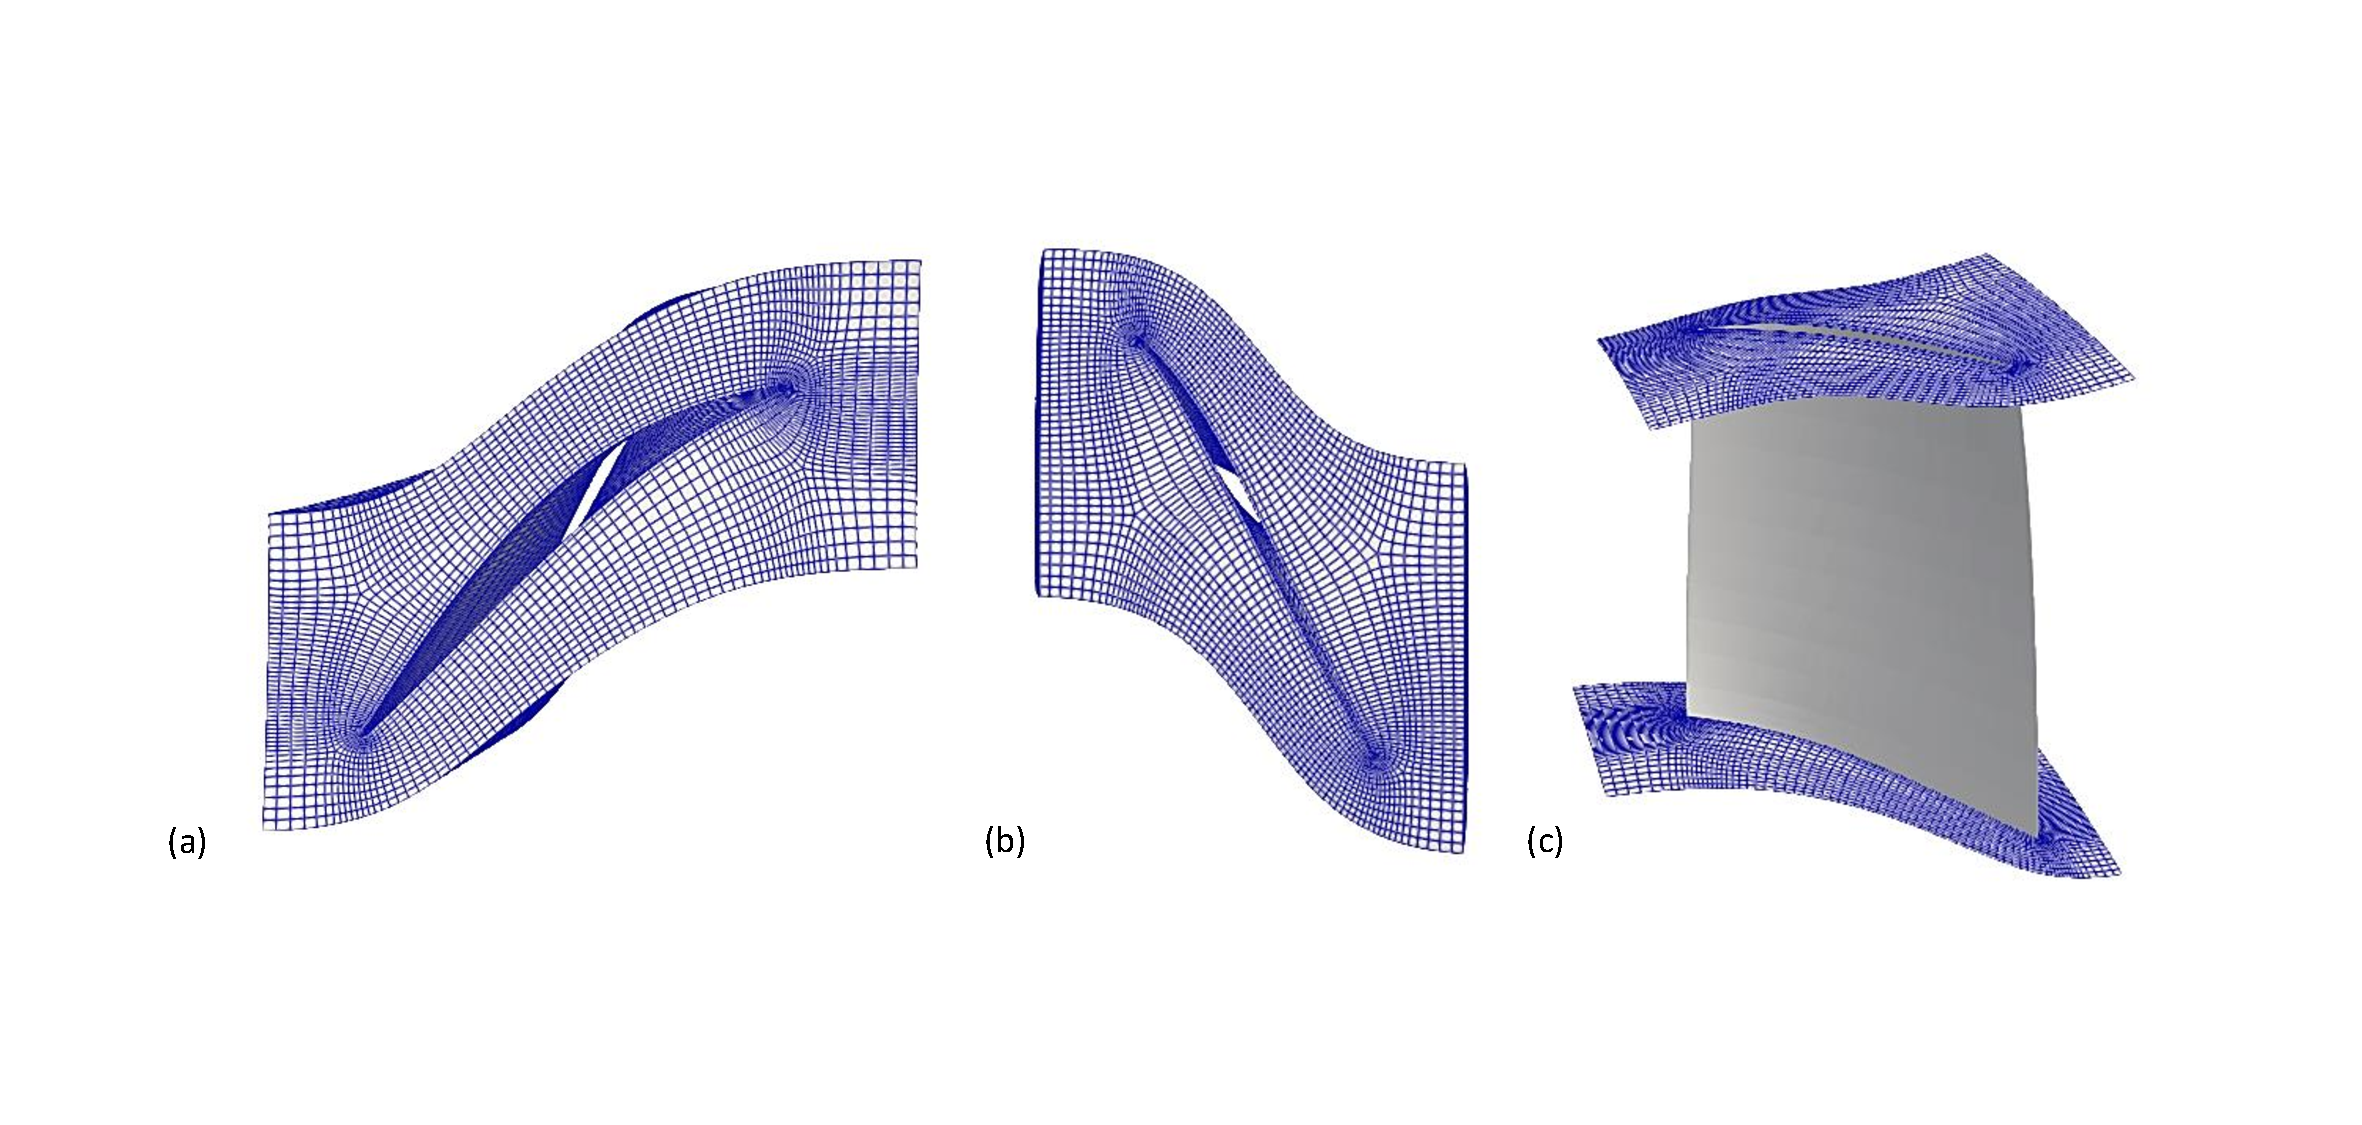
\includegraphics[width=1\linewidth]{chapter6/fig/fig_blade_simulation_mesh.pdf}
    \end{center}
    \caption{
        \small CFD mesh for efficiency validation: (a) hub view, (b) tip view, (c) side view.
    }
    \label{ch6:fig:blade_simulation_mesh}
\end{figure}

\begin{figure}[!htb]
    \begin{center}
        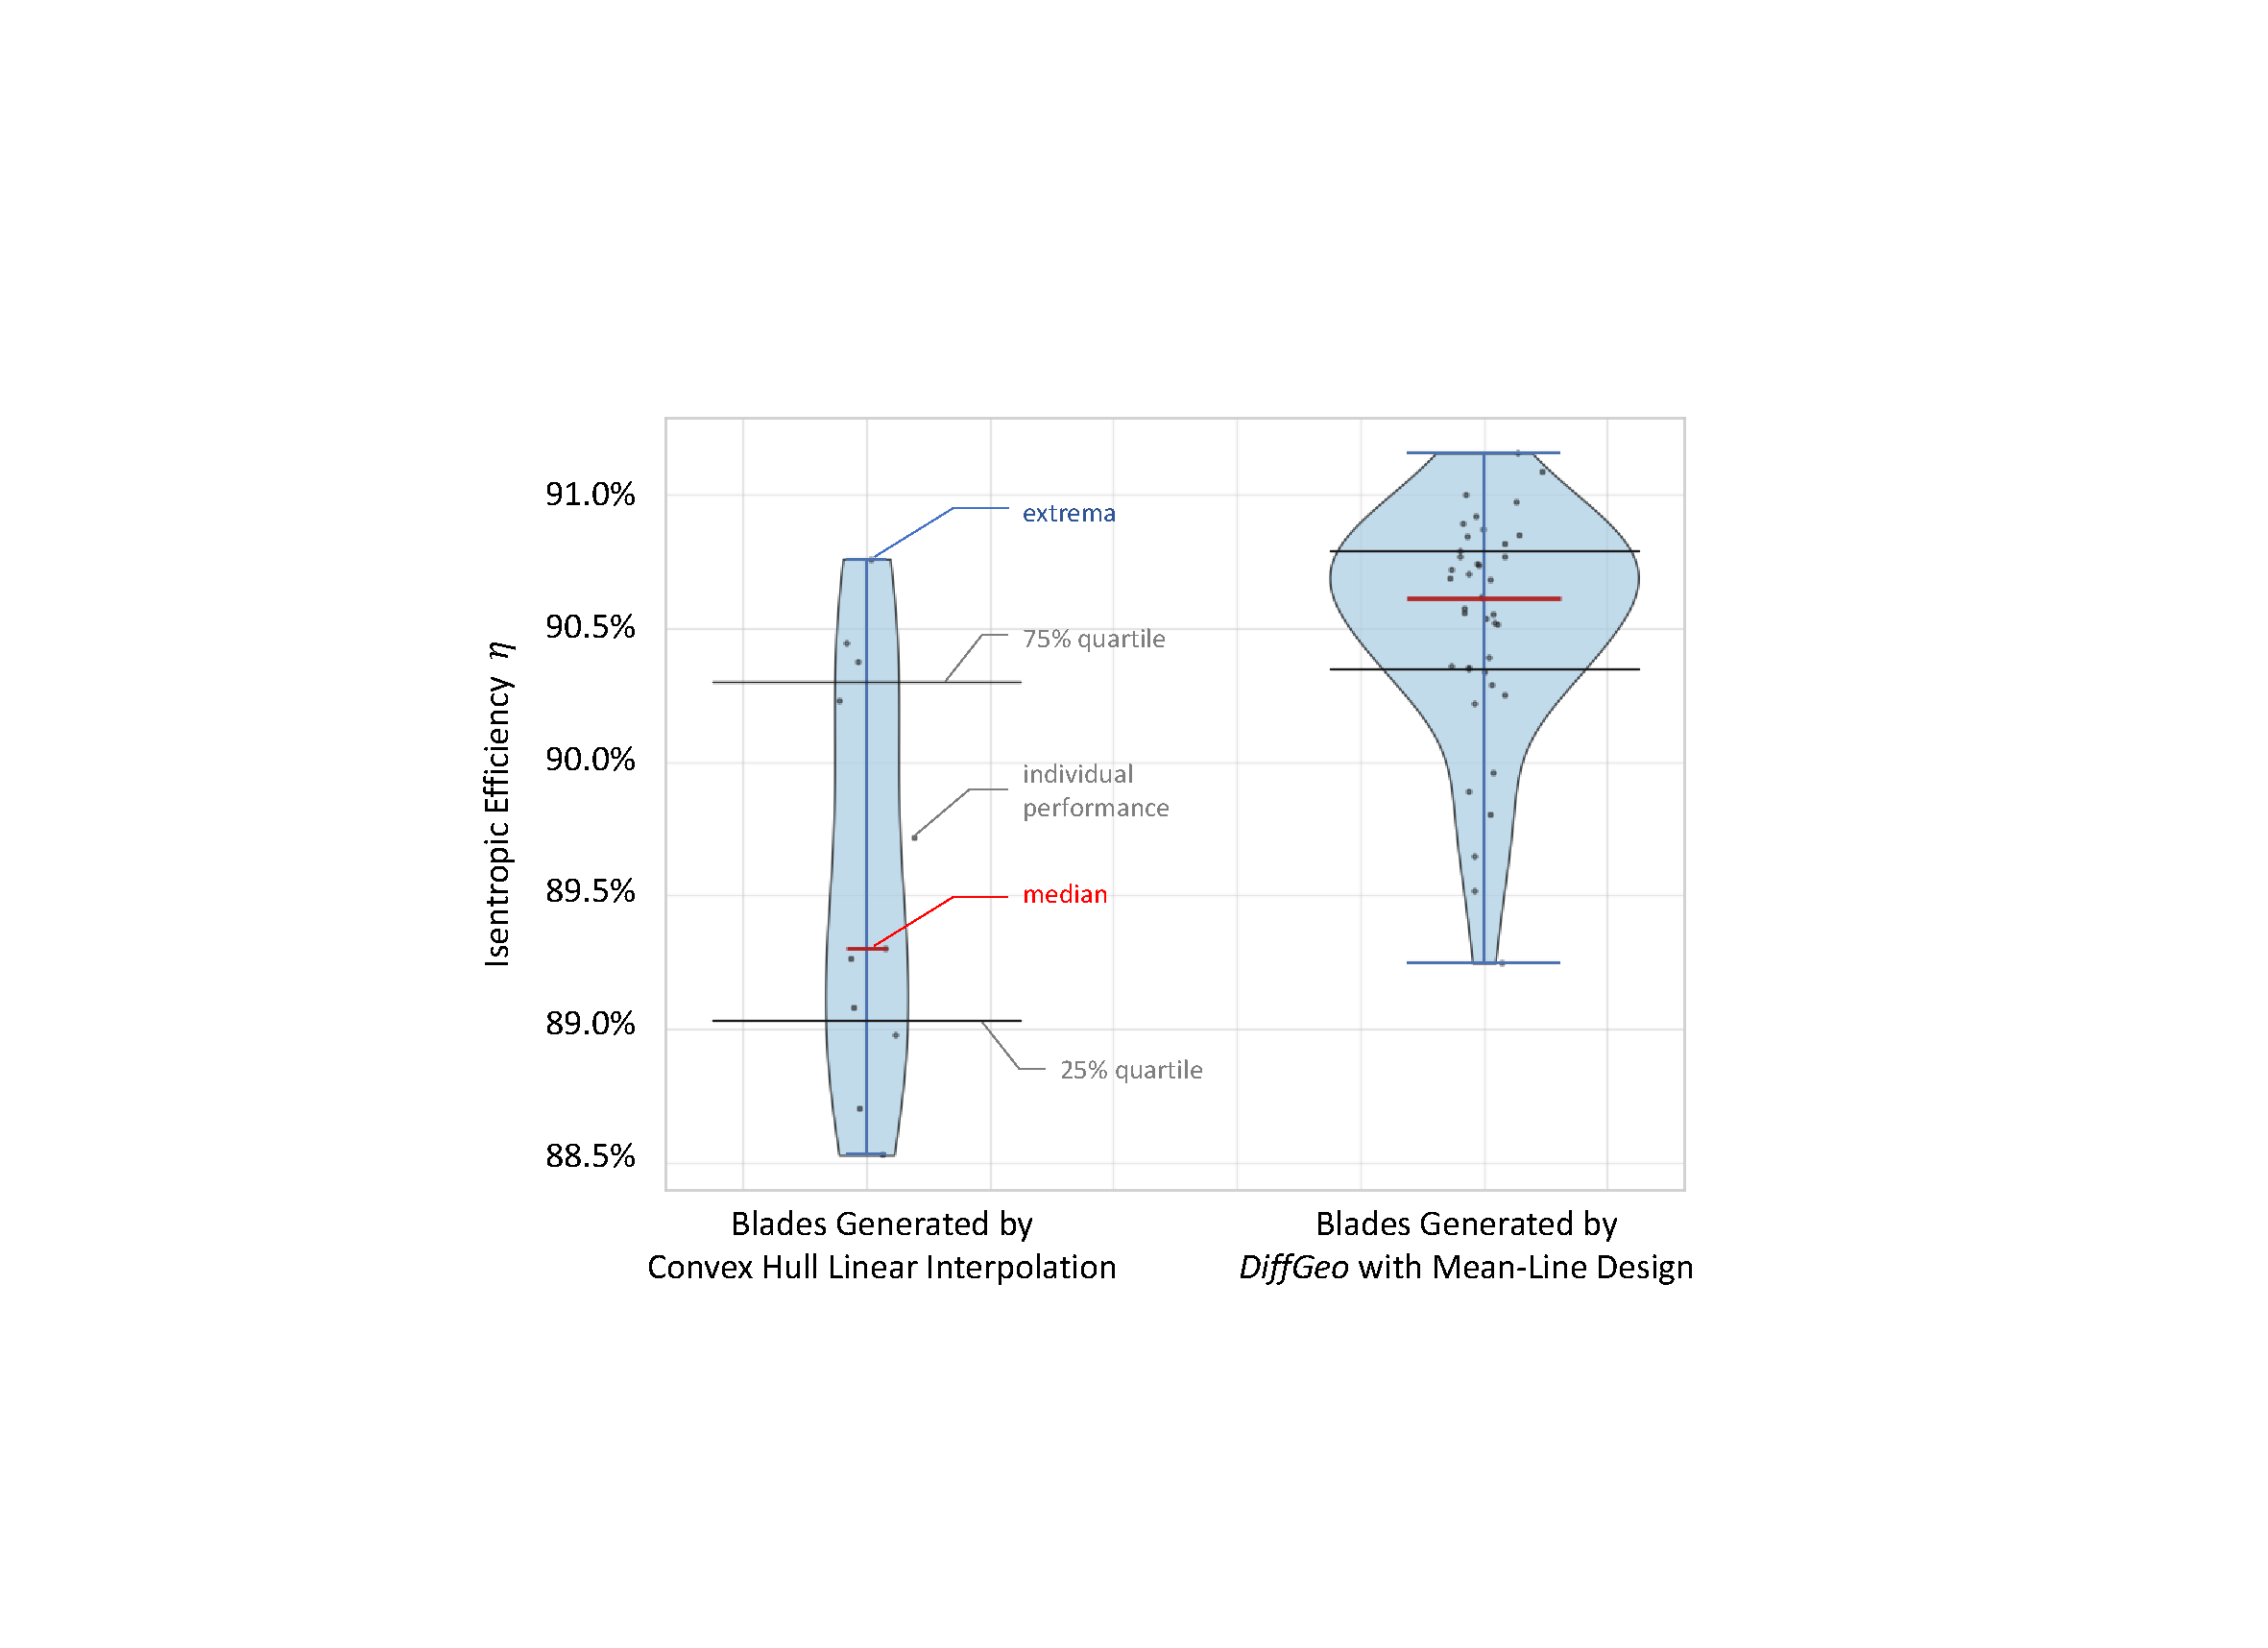
\includegraphics[width=1\linewidth]{chapter6/fig/fig_isentropic_efficiency.pdf}
    \end{center}
    \caption{
        \small Isentropic efficiency $\eta$ distributions for linearly convex-interpolated and conditional \textit{DiffGeo} blades.
    }
    \label{ch6:fig:isentropic_efficiency}
\end{figure}

One side effect of the strong twist guidance is that a fraction of the sampling can produce invalid shapes, accounting for $26\%$ of all samples. These invalid blades have less smooth surfaces when the latent code was pushed too far. However, this is not prohibitive since those invalid cases are easily filtered out with visual check or simple geometric validity check. As a result, 222 valid blades were left that meet the twist requirement. This $74\%$ success rate is still a favorable trade-off, given that producing a manually twist-aligned blade normally requires significant labor.

We then evaluate the aerodynamic performance of these blades through CFD simulations. To evaluate all blade profiles within a reasonable amount of time, we use a relatively lower-fidelity setup \footnote{\url{https://dafoam.github.io/mydoc_tutorials_aero_rotor37.html}} with DAFoam's RANS solver~\cite{aa.He2020}. Each profile is meshed by deforming from a template 40k-cell CFD mesh originally built on Rotor 37 that only models the blade passage (shown in Fig.~\ref{ch6:fig:blade_simulation_mesh}), by using the \textit{DeepGeo}~\cite{aa.Wei2024b,aa.Wei2025} model. The simulation produces shaft torque $C_{mz}$, pressure ratio $PR$, single-channel mass flow rate $\dot m$, from which we compute the isentropic efficiency $\eta$ defined as a ratio between the rotor's ideal work $W_{ideal}$ and actual work $W_{actual}$:
\begin{align}
    \eta &= \frac{W_{ideal}}{W_{actual}} \nonumber \\
         &= \frac{c_p\bigl(T_{0,out,ideal}-T_{0,in}\bigr)}{\frac{\omega \cdot C_{mz}}{\dot m}} \nonumber \\
         &= \frac{c_p \cdot T_{0,in} \cdot \bigl(\frac{p_{0,out}}{p_{0,in}}^\frac{\gamma-1}{\gamma}-1\bigr)}{\frac{\omega \cdot C_{mz}}{\dot m}}\\
         &= \frac{c_p \cdot T_{0,in} \cdot \bigl({PR}^\frac{\gamma-1}{\gamma}-1\bigr)}{\frac{\omega \cdot C_{mz}}{\dot m}}\;, \nonumber
\end{align}
where $\omega$ is the rotor’s rotation speed, $c_p$ the specific heat and $\gamma$ the specific heat ratio. $T_{0,in}$ and $T_{0,out,ideal}$ are the inlet total temperature and outlet ideal temperature, and $p_{0,in}$, $p_{0,out}$ are the corresponding total pressures. For comparison, we perform the same evaluation for the 75 convex hull interpolation blades in the training set. During this process, 193 generated blades and 55 dataset blades produce converged simulation results. The design candidates are selected if the blade's total pressure ratio close to the initial specifications (i.e. $1.6\geq {PR} \geq 1.58$), resulting in a selection of 45 generated blades ($20.3\%$ of valid generations) and 10 dataset blades (13.3\% of valid dataset profiles).

\begin{table}[htbp]
  \centering
  \caption{Sampling efficiency comparison between convex hull interpolation and \textit{DiffGeo} conditional sampling.}
    \begin{tabular}{lcc}
    \hline
    DSE Methods & Convex Hull Interpolation & DiffGeo + Mean Line Design \\
    \hline
    Number of Total Samples & 75     & 300 \\
    \hline
    Number and Ratio of  &        &   \\
    $\quad$ Valid Samples & 75 (100\%) & 222 (74.0\%) \\
    $\quad$ Successful Simulations & 55 (73.3\%) & 193 (86.9\%) \\
    $\quad$ Design Candidates & 10 (13.3\%) & 45 (20.3\%) \\
    \hline
    Isentropic Efficiency Median & 89.3\% & 90.7\% \\
    \hline
    \end{tabular}%
  \label{ch6:tab:turbine_sample}%
\end{table}%

Fig.~\ref{ch6:fig:isentropic_efficiency} summarizes the efficiency results. \textit{DiffGeo}-generated blades (on the right hand side) show consistently higher efficiency than the interpolated ones (on the left hand side). The median $\eta$ of the generated blades is about 90.7\%, whereas the convex hull interpolations’ median is 89.3\%. Additionally, the top end of the \textit{DiffGeo} efficiency range exceeds that of any interpolated blade. Statistics in Table~\ref{ch6:tab:turbine_sample} show that \textit{DiffGeo}’s conditional sampling guided by mean-line design outputs produces more valid designs, more high-performance candidates, and a higher median efficiency than the linear interpolation approach, even it starts from the same six baseline designs.

We also applied the linear convex-hull reconstruction test to the \textit{DiffGeo}-generated blades. The mean reconstruction error measured as averaged per-surface-point L2 distance is 5.9, indicating that the high-efficiency designs lie outside the convex hull of the bases. Their performance gains arise from nonlinear geometric variations in \textit{DiffGeo}’s latent space rather than from simple linear combinations of the base blades.

\subsubsection{Conclusions}
This 3D blade case study highlights several points that address the research questions raised at the beginning of this section.

First, \textit{DiffGeo} remains highly data-efficient in 3D. Even though trained on the linear convex hull derived from only six blades, \textit{DiffGeo} learns a valid 3D design manifold without requiring extensive databases. This data setup reflects a realistic engineering constraint where only a limited number of existing designs are available. Traditional deep generative models such as GANs and VAEs would struggle under the same condition and typically require thousands of geometries to ensure stable training.

Second, \textit{DiffGeo} is proved flexible and reusable. We used the same trained model to handle different objectives, including enforcing thickness constraints and matching a twist law, all without retraining. This demonstrates the power of having a task-agnostic generative model that can be guided as needed. It opens up possibilities for integrating physics-based extensions, such as incorporating adjoint solvers, directly into the generative process, without needing to repeat the expensive data collection for each new requirement.

Third, \textit{DiffGeo} can handle complex engineering constraints in generation. It can satisfy spatially varying constraints that would be difficult to enforce via conventional statistical sampling or by training a classifier-free conditional generator. By combining \textit{DiffGeo} with classical design tools, we demonstrate a new workflow that directly injects expert knowledge into generative design, producing feasible and high-performing designs with minimal manual effort. 

Notably, this case study shows that \textit{DiffGeo} goes beyond interpolating known shapes, as it generates truly novel blade geometries that lie outside the linear convex hull defined by the training data. This is quantitatively verified by the reconstruction error analysis, where generated blades deviate from the linear data space by several orders of magnitude. These novel designs also exhibit higher isentropic efficiencies than any interpolated baseline blade, which highlights \textit{DiffGeo}’s creative extrapolation capability. Rather than replicating historical shapes, it discovers new and high-performing designs, demonstrating both generalization beyond data and the practical advantage for design space exploration.